% ---------------------
% GRAPHIQUES ET FIGURES
% ---------------------

% Defining TOC's sections before content
\section{Graphiques et figures}

\begin{frame}
    \vfill
    \begin{center}
        \large
        Graphiques et figures
    \end{center}
    \vfill
\end{frame}

\begin{frame}
    \frametitle{Graphiques et figures}
    Un module pratique pour la mise en page de figures est \textcolor{hard_green}{\textit{subfloat}}\footnotemark. Celle-ci permet de mettre plusieurs sous-figures dans un même environnement.
    \vfill
    \begin{figure}
        \centering
        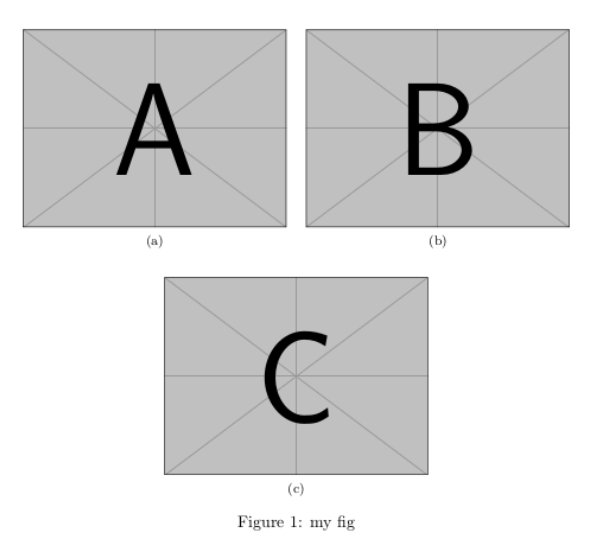
\includegraphics[width=0.4\linewidth]{LATEX_CONF_2024_10_02/figures/subfloat.png}
        \label{fig: subfloat}
    \end{figure}
    \footnotetext{subfloat – Sub-numbering for figures and tables. \href{https://ctan.org/pkg/subfloat}{\textcolor{spruce_dark}{https://ctan.org/pkg/subfloat}}.}
\end{frame}

\begin{frame}
    \frametitle{Graphiques et figures}
    Un autre module utile pour la mise en page de figures est \textcolor{hard_green}{\textit{wrapfig}}\footnotemark. Celle-ci permet d'insérer une figure à l'intérieur d'une zone de texte.
    \vfill
    \begin{figure}
        \centering
        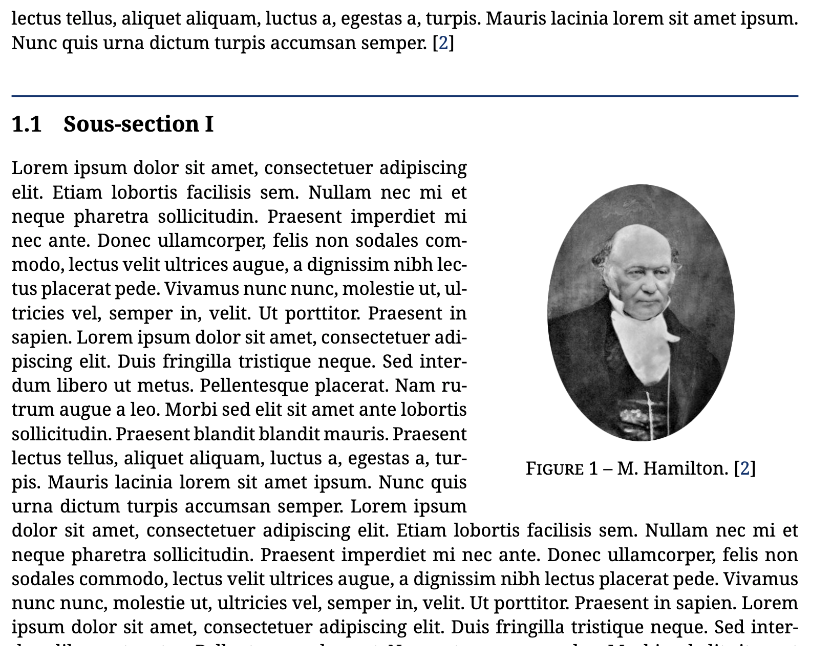
\includegraphics[width=0.45\linewidth]{LATEX_CONF_2024_10_02/figures/wrapfig.png}
        \label{fig: wrapfig}
    \end{figure}
    \footnotetext{wrapfig – Produces figures which text can flow around. \href{https://ctan.org/pkg/wrapfig}{\textcolor{spruce_dark}{https://ctan.org/pkg/wrapfig}}.}
\end{frame}

\begin{frame}
    \frametitle{Graphiques et figures}
    Il existe même un module qui permet de créer ses propres figures \textit{vectorisées} nommée \textcolor{hard_green}{\textit{TikZ}}\footnotemark
    \vfill
    \pause
    \begin{columns}
        \column{0.33\linewidth}
        \begin{figure}
            \centering
            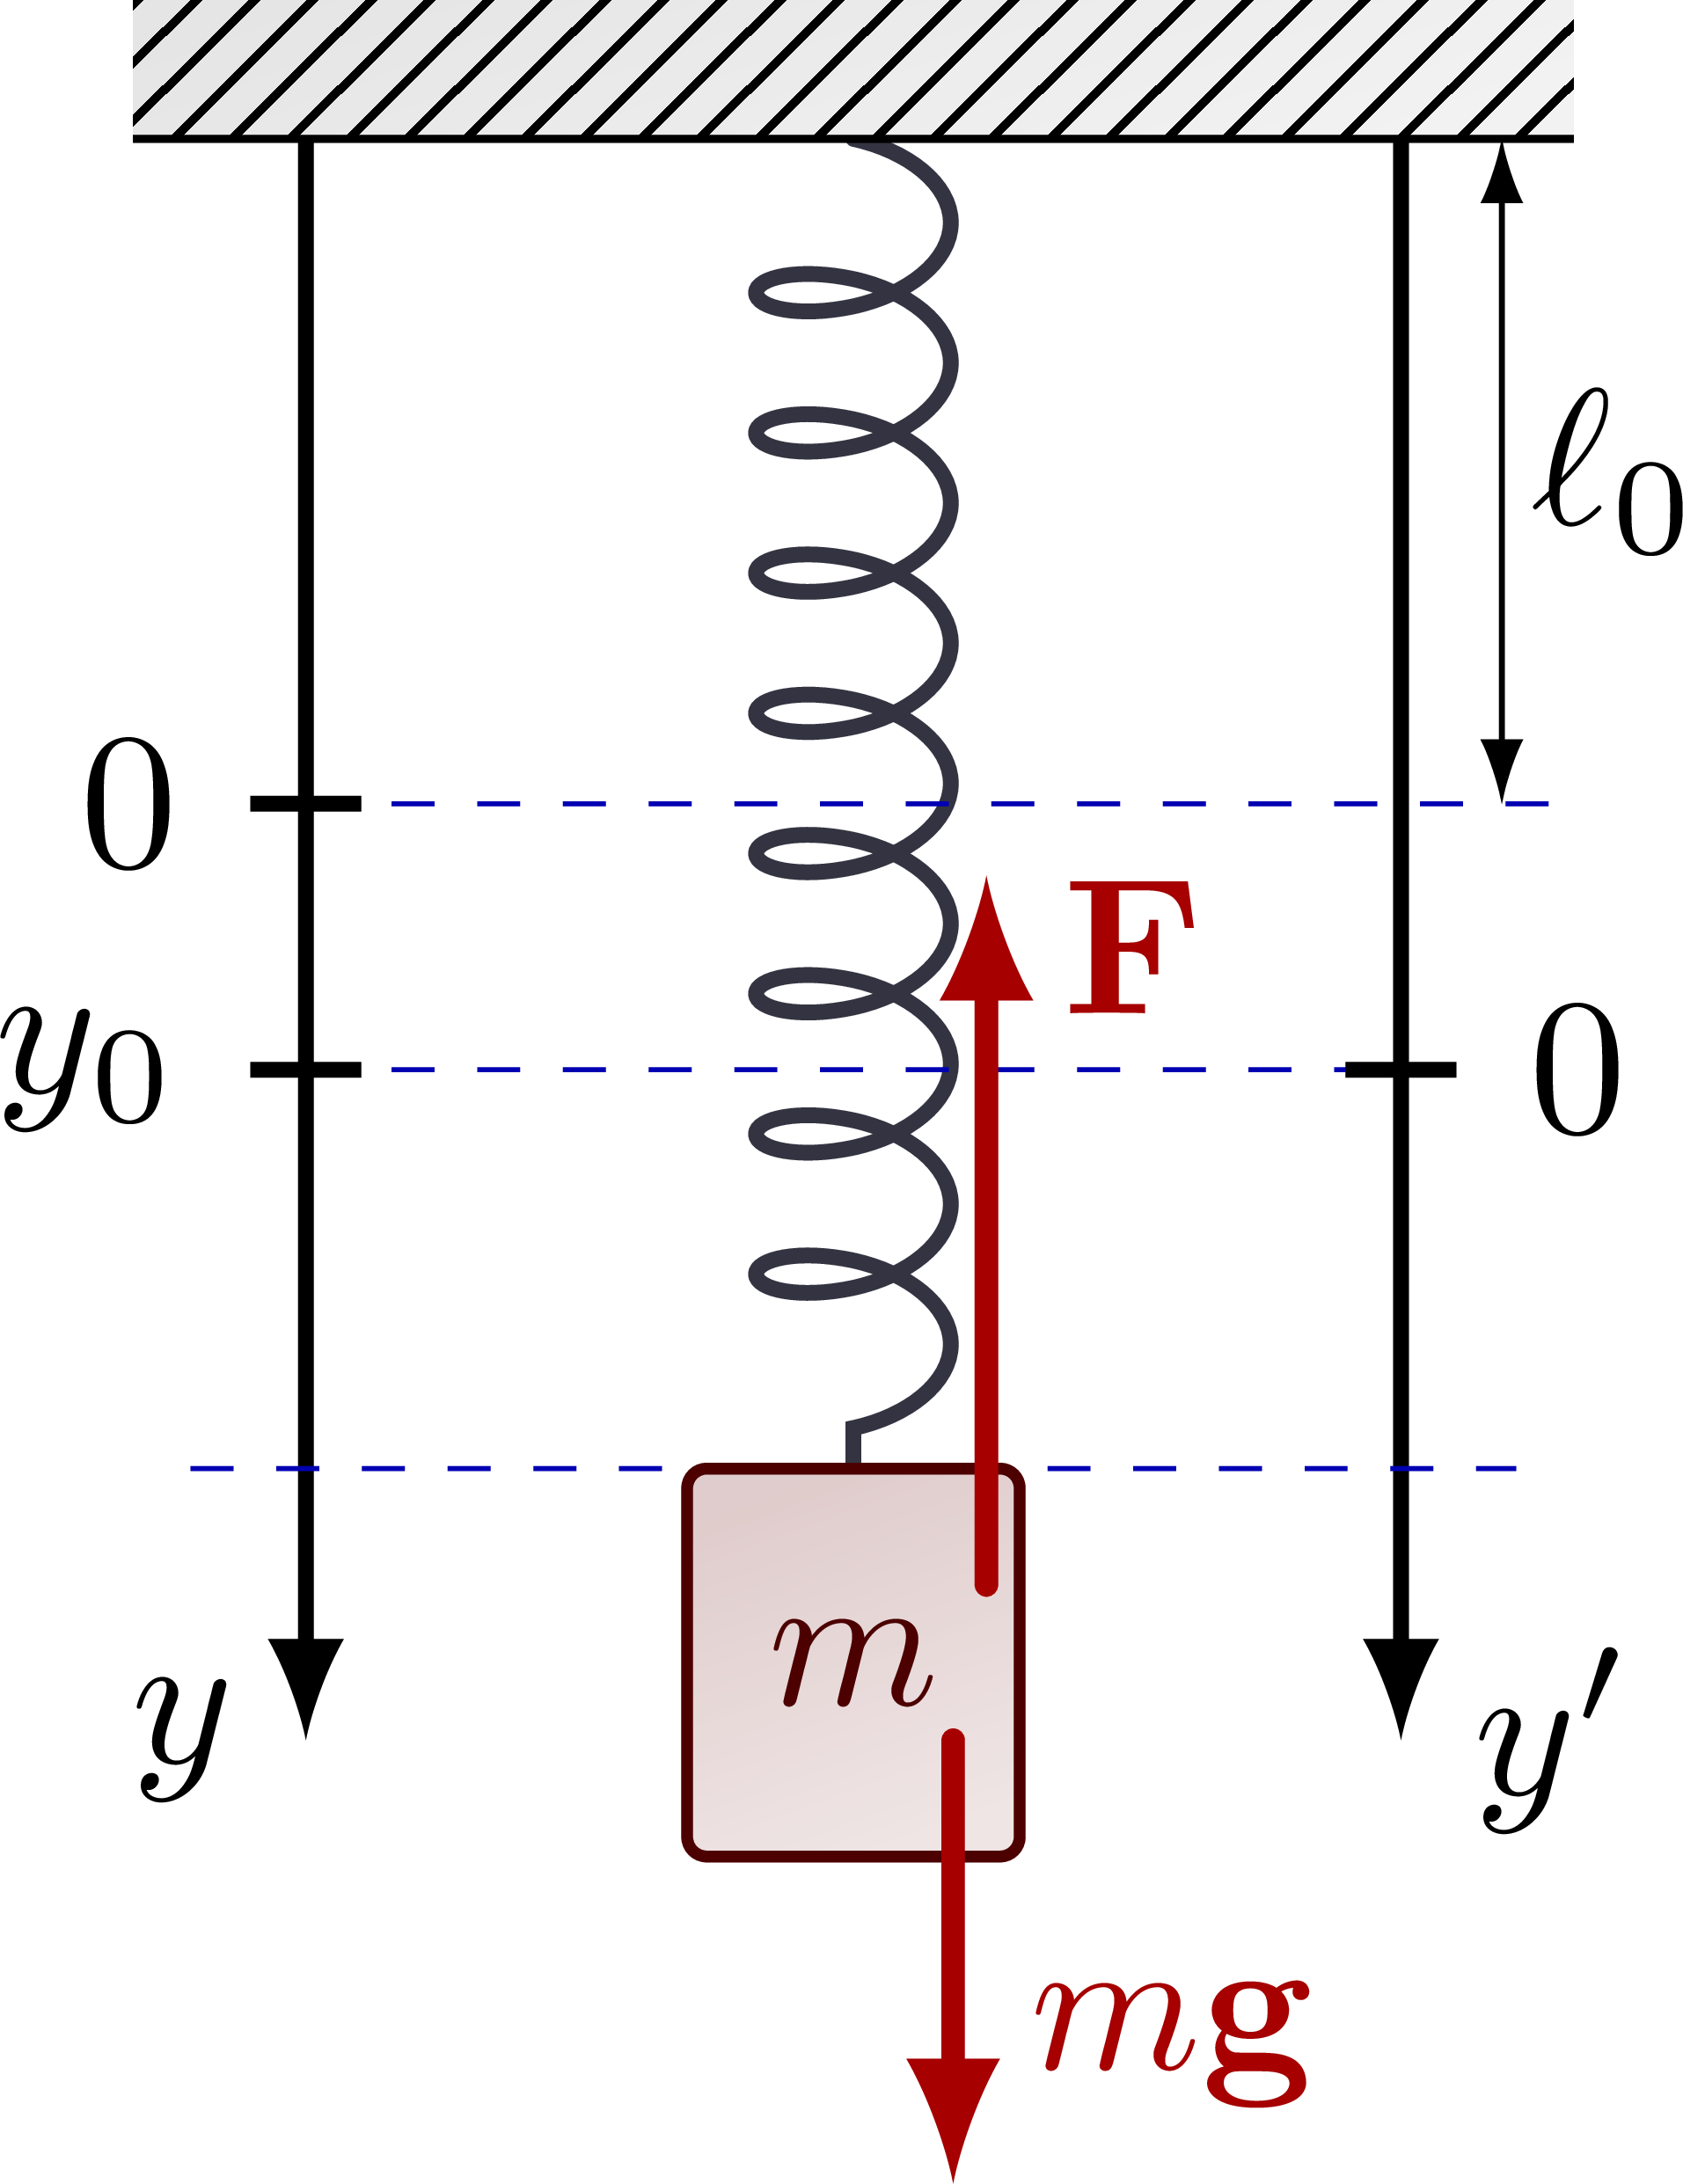
\includegraphics[width=0.55\linewidth]{LATEX_CONF_2024_10_02/figures/tikz.png}
            \label{fig: tikz}
        \end{figure}
        \column{0.33\linewidth}
        \pause
        \begin{figure}
            \centering
            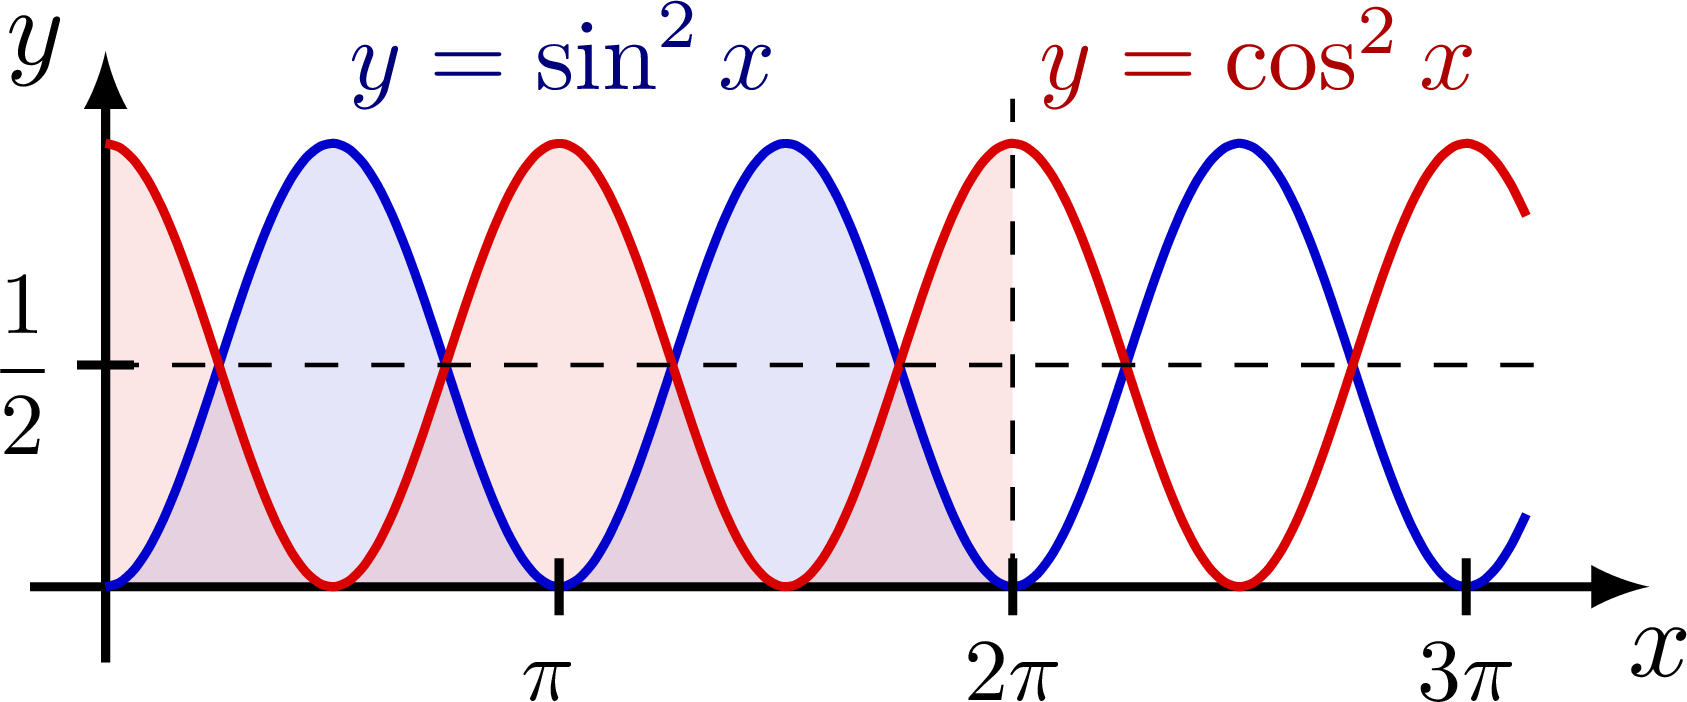
\includegraphics[width=0.9\linewidth]{LATEX_CONF_2024_10_02/figures/tikz_2.png}
            \label{fig: tikz}
        \end{figure}
        \column{0.33\linewidth}
        \pause
        \begin{figure}
            \centering
            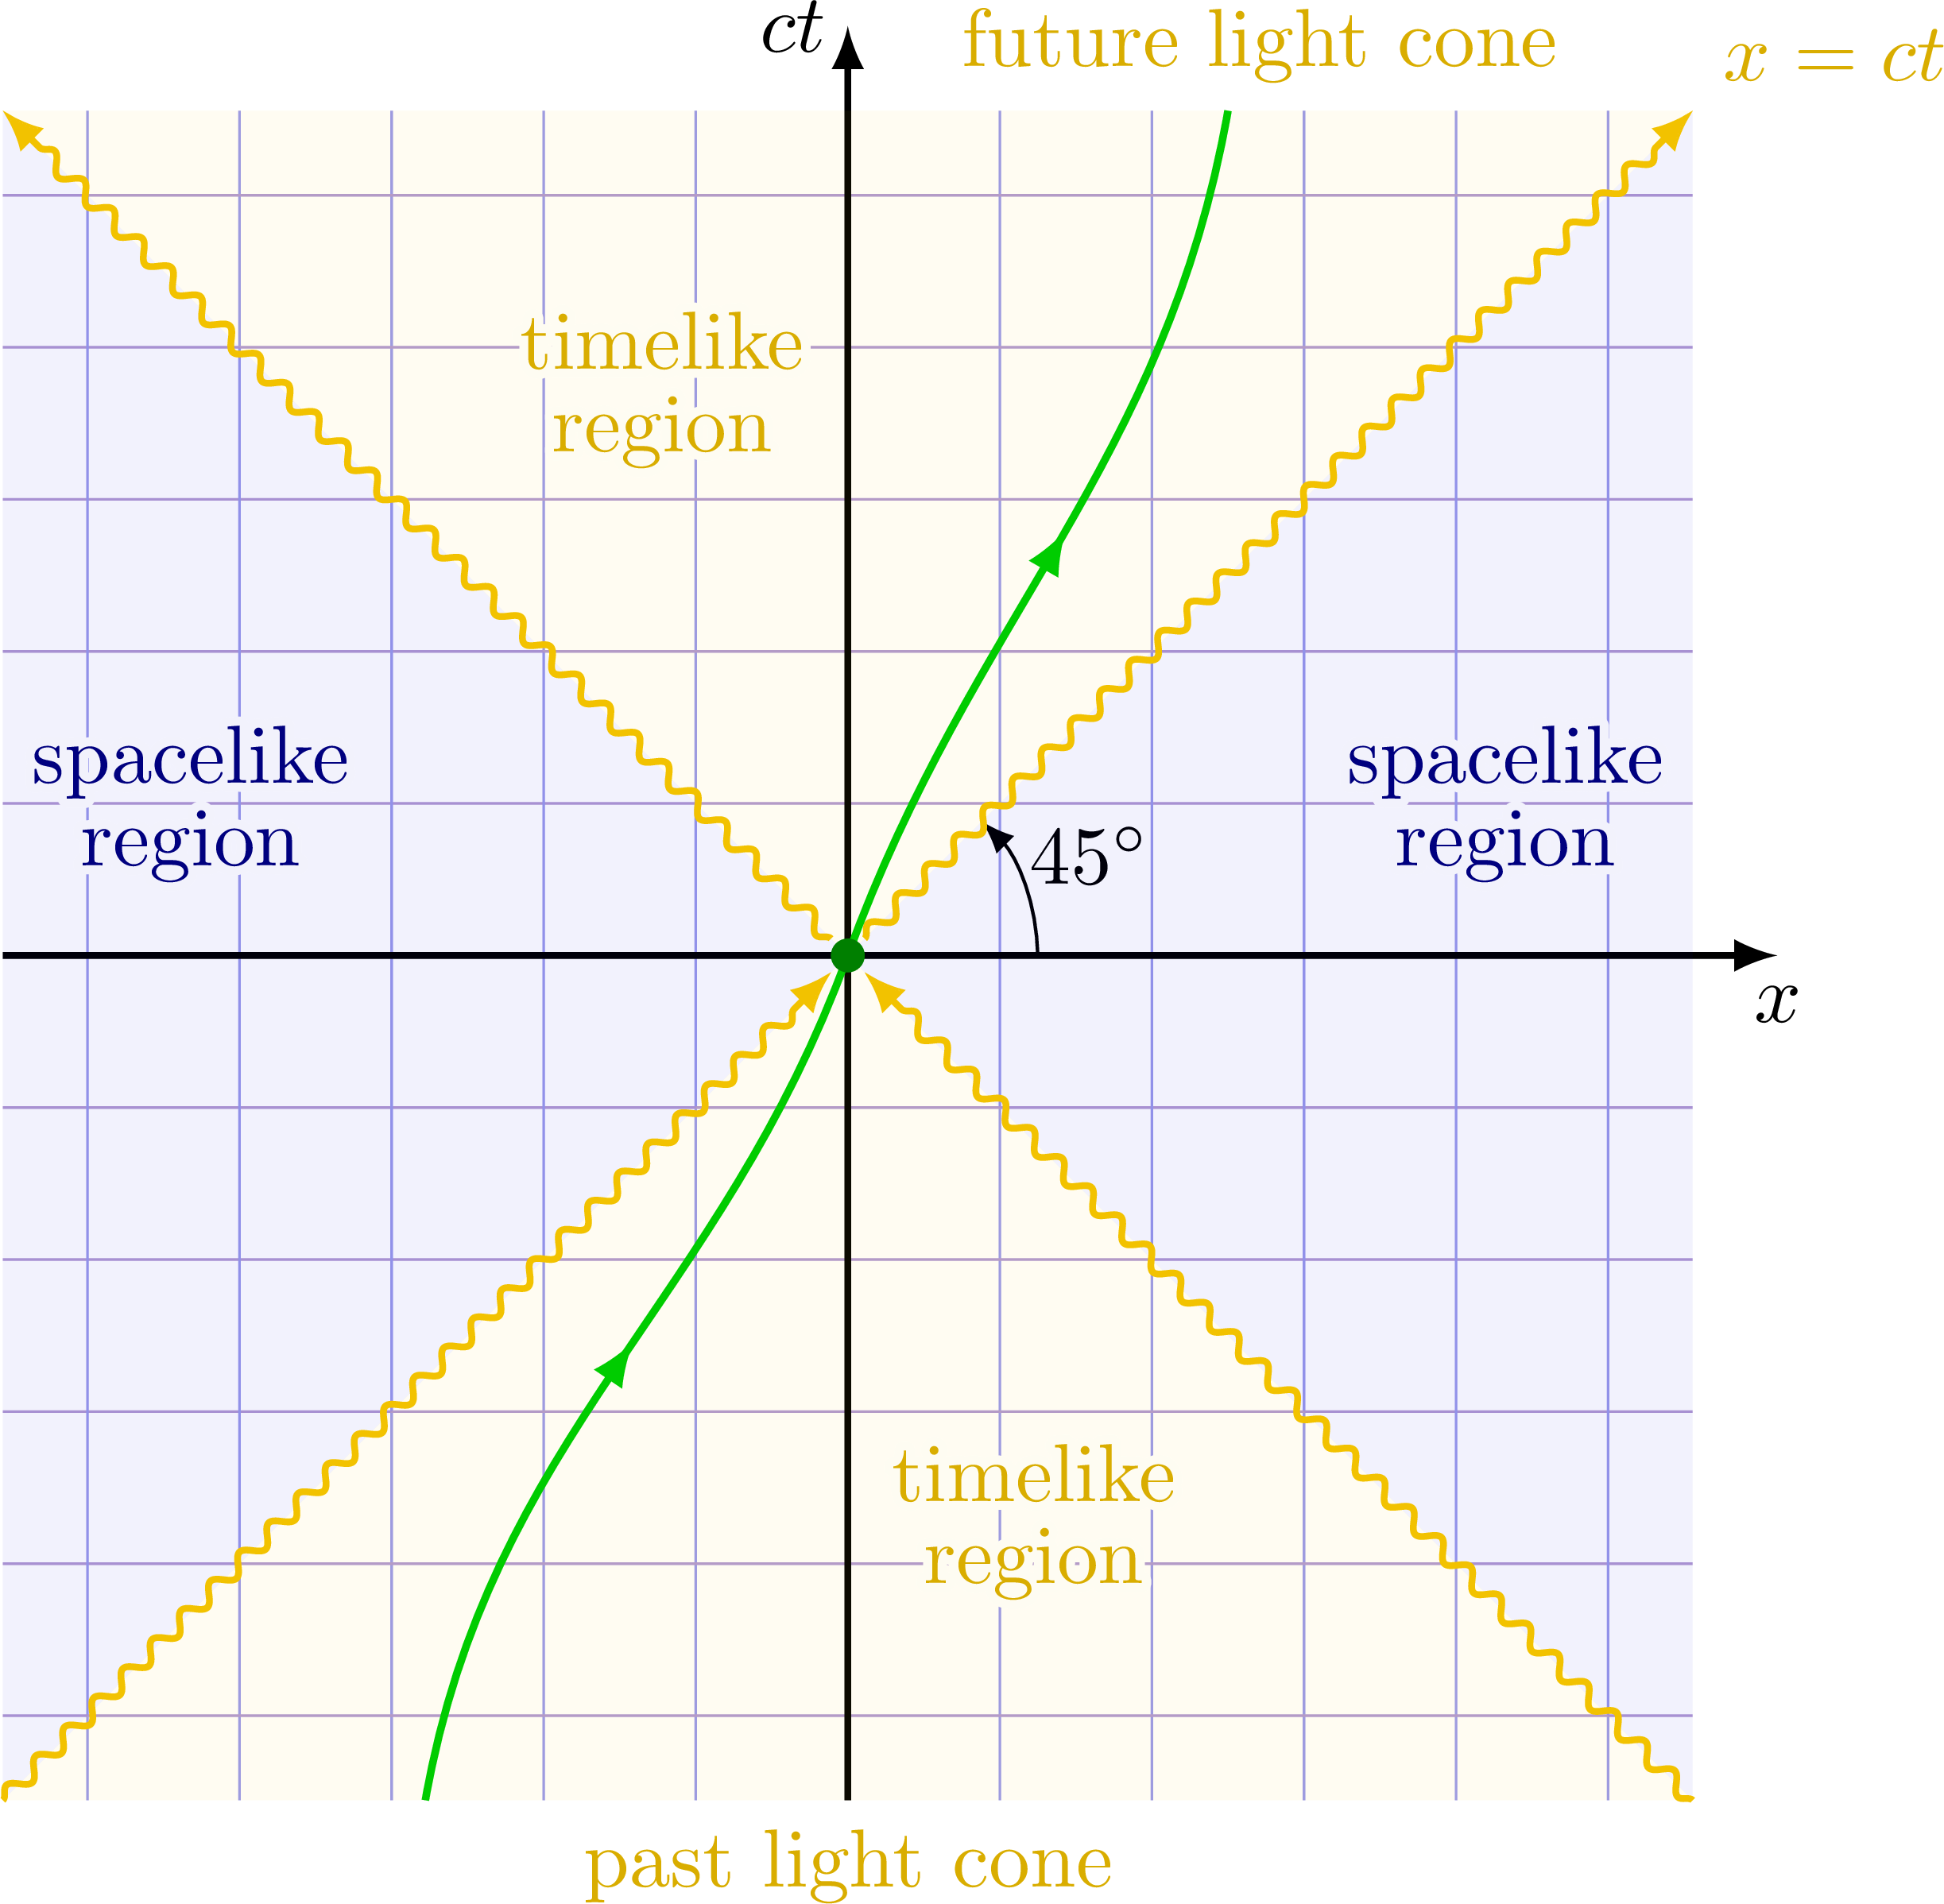
\includegraphics[width=0.85\linewidth]{LATEX_CONF_2024_10_02/figures/tikz_3.png}
            \label{fig: tikz}
        \end{figure}
    \end{columns}
    \vfill
    \footnotetext{pgf – Create PostScript and PDF graphics in \TeX. \href{https://www.ctan.org/pkg/pgf}{\textcolor{spruce_dark}{https://www.ctan.org/pkg/pgf}}.}
\end{frame}